%%
\bigheading{Next Permutation}
\authors{Gyula Horváth}{Gyula Horváth}{Gyula Horváth}
%%
\heading{Naive solution}
Algorithm: Take next permutation until 3-1-2 avoiding permutation found.\\
The running time of this algorithm is exponential in worth case, since there is a 3-1-2 avoiding permutation $\pi$ of $n$ elements such that there are $(n-2)!-1$ permutations between $\pi$ and the next 3-1-2 avoiding permutation. For example, if $\pi=\langle n-1,n,n-2,\ldots, 2,1 \rangle$ then the next 3-1-2 avoiding permutation is $\langle n,n-1,n-2,\ldots , 2,1 \rangle$.
\heading{Linear time solution}
First we show that 3-1-2 avoiding permutations can be represented by stack generation. Consider the following stack operations\\
\begin{center}
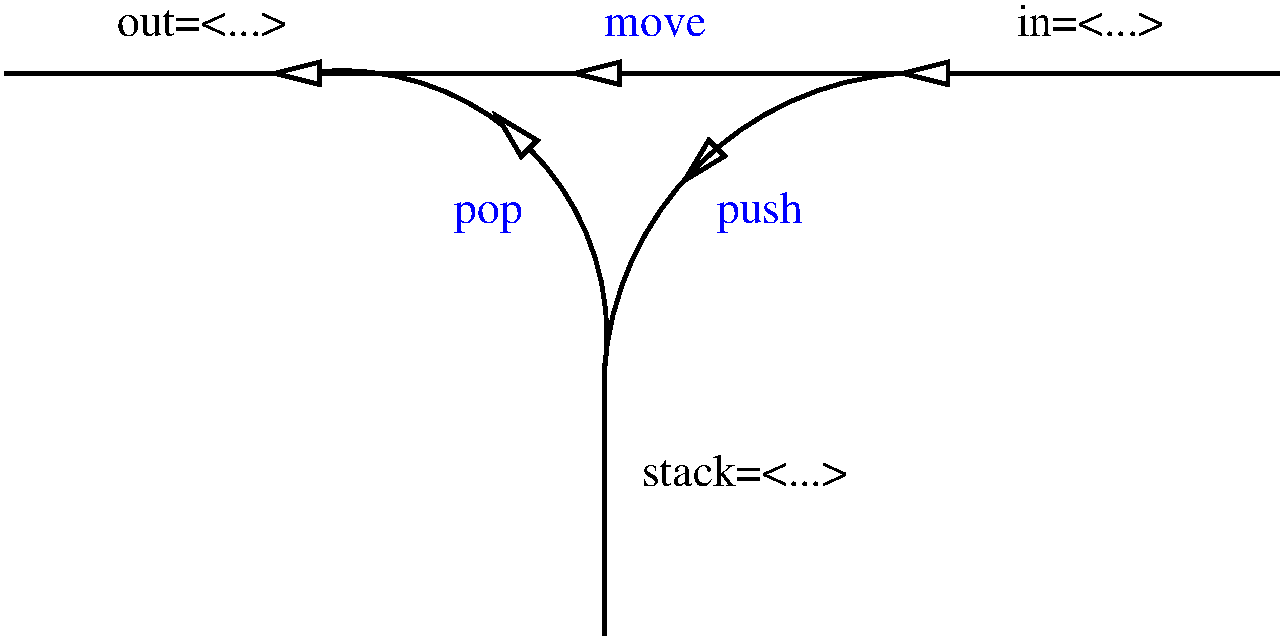
\includegraphics[height=4cm]{img/vasut.pdf}
\end{center}
%\hrule
\subsubsection*{I/O specification of the stack operations}
\begin{eqnarray}
\{in=\langle a,\alpha \rangle \wedge  stack=\langle \beta \rangle \wedge  out=\langle \gamma \rangle\} & move & \{ in=\langle \alpha\rangle \wedge  stack=\langle\beta \rangle \wedge  out=\langle \gamma,a \rangle\}\\
\{ in=\langle a,\alpha \rangle \wedge  stack=\langle \beta \rangle \wedge  out=\langle\gamma \rangle\} & push & \{ in=\langle\alpha \rangle stack=\langle \beta,a \rangle \wedge  out=\langle\gamma  \rangle\}\\
\{ in=\langle \alpha \rangle \wedge  stack=\langle\beta,b \rangle \wedge  out=\langle\gamma \rangle\} & pop & \{ in=\langle\alpha \rangle \wedge  stack=\langle\beta \rangle \wedge out=\langle \gamma,b \rangle  \}
\end{eqnarray}
We say that a permutation $\pi$ can be generated by stack if there is a sequence of stack operations that results $\pi$ from the input sequence $\langle1,2, \ldots , n \rangle$.
\subsubsection*{Statement}
A permutation $\pi$ is a 3-1-2 pattern avoiding permutation if and only if $\pi$ can be generated by stack.
\subsubsection*{Proof}
Assume that $\pi$ is generated by stack. Consider the moment when an element $x$ moved to the output (by move or pop operation). In this  moment every element of the input sequence larger then $x$, moreover, the stack content is always decreasing sequence. Therefore there is no 3-1-2 pattern in $\pi$ with $x$ as the first element of the pattern.

Conversely, we prove by induction on the length of the permutation that every 3-1-2 pattern avoiding permutation can be generated by stack. It is obvious that every permutation of length 1 or 2  can be generated by stack. Consider a 3-1-2 pattern avoiding permutation $\pi$ of the elements $1,\ldots, n$ and decompose it as $\pi =\langle \alpha,1,\beta \rangle$. Both $\alpha$ and $\beta$ are 3-1-2 pattern avoiding sequence. Moreover, due to the 3-1-2 pattern avoiding property, if $k$ is the largest element of $\alpha$ then $\alpha$ contains all numbers from $2$ to $k$. Consequently, $\beta$ contains all numbers from $k+1$ to $n$. By induction, $\alpha$ can be generated by stack with a sequence of stack operations $(\alpha)$ from the input sequence $2,\ldots,k$. Similarly, $\beta$ can be generated with a sequence of stack operations $(\beta)$ from the sequence $k+1,\ldots,n$. Therefore, the sequence of stack operations $push,(\alpha),pop,(\beta)$ generates $\pi$ from the input sequence $\langle1,2,\ldots,k,k+1,\ldots, n \rangle$.\\

Notice that the generating sequence of stack operations is unique if $push;pop$ not allowed (give $move$ instead).\\
Let $\pi$ be a 3-1-2 pattern avoiding permutation of length $n$. Decompose $\pi$ according to the position of the number $n$ in $\pi$: $\pi=\langle\pi_1,u,n,\pi_2 \rangle$. The position of  $u$ is the largest position such that there is a larger element than $u$ in the sequence whose position is larger than the position of $u$. Consider the moment of the stack generation of $\pi$, when $u$ moved (by $move$ or $pop$ operation) to the output:
\[out=\langle \alpha,u \rangle \textrm{ and }  in=\langle\beta \rangle \textrm{ and } stack=\langle\gamma \rangle\],
where $\beta=v,v+1,\ldots,n$ for some $v$. Then
\[\pi=\langle\alpha,u,\textrm{mirror}(\beta), \textrm{mirror}(\gamma) \rangle\]
The permutation
 \[\rho=\langle \alpha,v,u,\textrm{mirror}(\gamma), v+1,\ldots, n \rangle\]
  is a 3-1-2 pattern avoiding permutation because $\rho$ can be generated by stack, and $\rho$ follows $\pi$ according to the lexicographic ordering since $u<v$. Moreover, all elements of $\gamma$ are less than $u$ and $v$ is the smallest in $\beta$ implies that there is no 3-1-2 pattern avoiding permutation between $\pi$ and $\rho$. \\


Using this observation we can develop $O(n)$ running time algorithm which computes the next 3-1-2 avoiding permutation.
